\documentclass[conf]{new-aiaa}
%\documentclass[journal]{new-aiaa} for journal papers
\usepackage[utf8]{inputenc}

\usepackage{graphicx}
\usepackage{amsmath}
\usepackage{commath}
\usepackage[version=4]{mhchem}
\usepackage{siunitx}
\usepackage{longtable,tabularx}
\usepackage{float}
\usepackage{listings}
\usepackage{pdfpages}
\usepackage{color} %red, green, blue, yellow, cyan, magenta, black, white
\definecolor{mygreen}{RGB}{28,172,0} % color values Red, Green, Blue
\definecolor{mylilas}{RGB}{170,55,241}
\setlength\LTleft{0pt} 

\lstset{language=Matlab,%
	basicstyle=\footnotesize,
	breaklines=true,%
	morekeywords={matlab2tikz},
	keywordstyle=\color{blue},%
	morekeywords=[2]{1}, keywordstyle=[2]{\color{black}},
	identifierstyle=\color{black},%
	stringstyle=\color{mylilas},
	commentstyle=\color{mygreen},%
	showstringspaces=false,%without this there will be a symbol in the places where there is a space
	numbers=left,%
	numberstyle={\tiny \color{black}},% size of the numbers
	numbersep=9pt, % this defines how far the numbers are from the text
	emph=[1]{for,end,break},emphstyle=[1]\color{red}, %some words to emphasise
	%emph=[2]{word1,word2}, emphstyle=[2]{style},    
}

% ================================================================ % 
\title{ASE387P.2 Mission Analysis and Design \\ Homework 3}

\author{Junette Hsin}
\affil{Masters Student, Aerospace Engineering and Engineering Mechanics, University of Texas, Austin, TX 78712}

\begin{document}

\maketitle

% \begin{abstract}

	% Theory and algorithms 

% \end{abstract}

% \newpage 
% ================================================================ % 
\section*{Problem 1}

\textbf{All analyses for this section are for a desired 60 degree transfer angle in the clockwise direction from the initial / departure position.} \\ 

The desired transfer angle of 60 degrees was defined to be the angle between the initial / departure longitude and the final / arrival longitude. 

\begin{equation}
    \Delta L_{des} = L_{M_f} - L_{E_i}
    \label{eq:DL}
\end{equation}

For an outbound transfer, the initial longitude would be Earth and the final longitude would be Mars. For inbound transfer, the initial longitude would be Mars and the final longitude would be Earth. Equation \ref{eq:DL} could also be rewritten as: 

\begin{equation}
    L_{M_f} = \Delta L_{des} + L_{E_i}
    \label{eq:Lf1}
\end{equation}

The final longitude can also be found from the motion of the planets: 

\begin{equation}
    L_{M_f} = L_{M_i} + \Delta t \dot{L_{M}}
    \label{eq:Lf2}
\end{equation}

Combing Equations \ref{eq:Lf1} and \ref{eq:Lf2} result in: 

\begin{equation}
    \Delta t = \frac{\Delta L_{des} + L_{E_i} - L_{M_i}}{ \dot{L_M} }
\end{equation}

The document \textbf{aprx\_pos\_planets.pdf} was used to compute the orbital elements and Cartesian states of Earth and Mars. Once $\Delta t$ and an initial time are known, the positions of the planets are known. 


% ------------------------- % 
\subsection*{A}

To calculate the synodic period, first, the period of Mars was calculated in years: 

\begin{equation}
    T_{Mars} = \frac{1}{\dot{L}_{Mars}} \times \frac{100 \; years}{1 \; century} \times \frac{360 ^\circ}{1 \; rev}
\end{equation}

The synodic period was then calculated with the following equation: 

\begin{equation}
    SP_{Mars} = \frac{T_{Mars}}{|| T_{Mars} - 1 ||}
\end{equation}

The synodic period came out to be 2.13526965089401. 

% ------------------------- % 
\subsection*{B}

The initial date was set to 2451545.0 JD. \\ 

The first date for 60 degree phasing was computed to be 2451859.90006635. \\ 

The time of flight for the minimum energy transfer conic was computed to be 174.476913251305 days for the short path and 202.984519445264 days for the long path. \\  

\begin{figure}[H]
    \centering 
    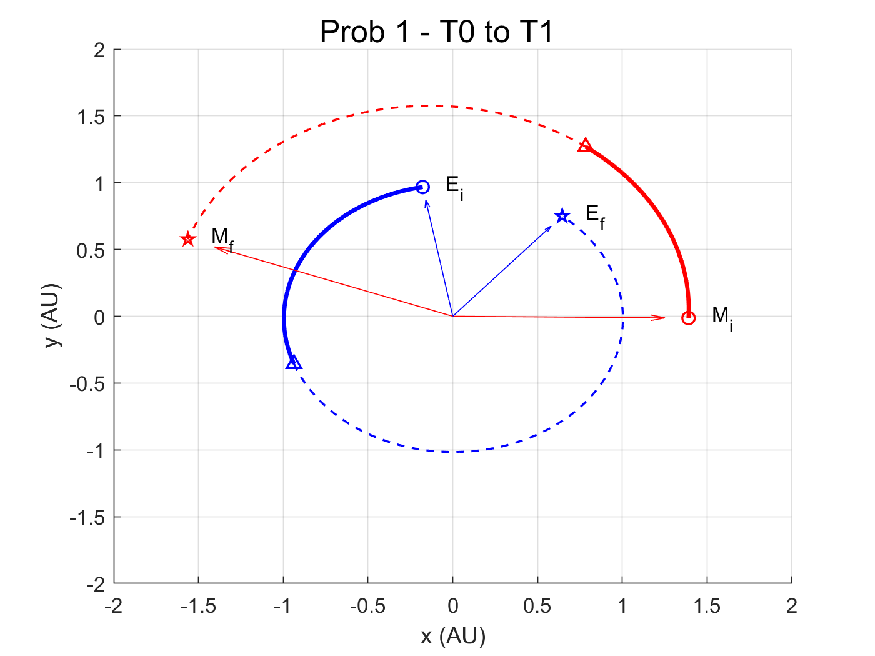
\includegraphics[width=0.7\textwidth]{Prob 1 - T0 to T1.pdf}
    \caption{1st Earth to Mars 60 degrees transfer}
\end{figure}

The second date for 60 degree phasing was computed to be 2452452.16890137 JD. \\ 

The time of flight for the minimum energy transfer conic was computed to be 206.969049395779 days for the long path and 184.202367869194 days for the short path. \\ 

\begin{figure}[H]
    \centering 
    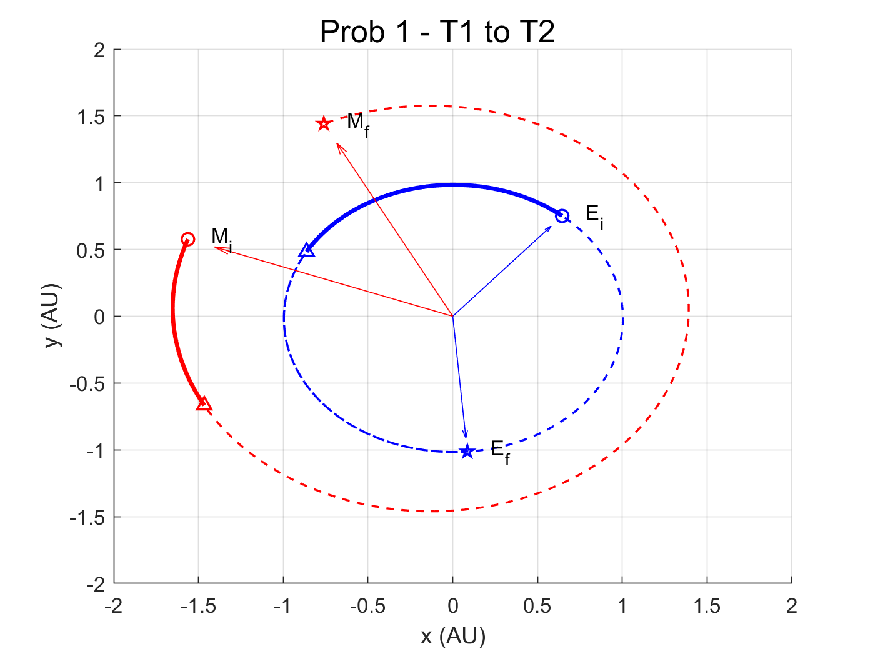
\includegraphics[width=0.7\textwidth]{Prob 1 - T1 to T2.pdf}
    \caption{2nd Earth to Mars 60 degrees transfer}
\end{figure}

% ------------------------- % 
\subsection*{C}

The date for 60 degree phasing inbound transfer was computed to be 
2452712.16492299 JD. From the previous outbound date, the wait time is 260 days. \\ 

The time of flight for the minimum energy transfer conic was computed to be 195.61527956253 days for the long path and 163.801713161463 days for the short path. \\ 

\begin{figure}[H]
    \centering 
    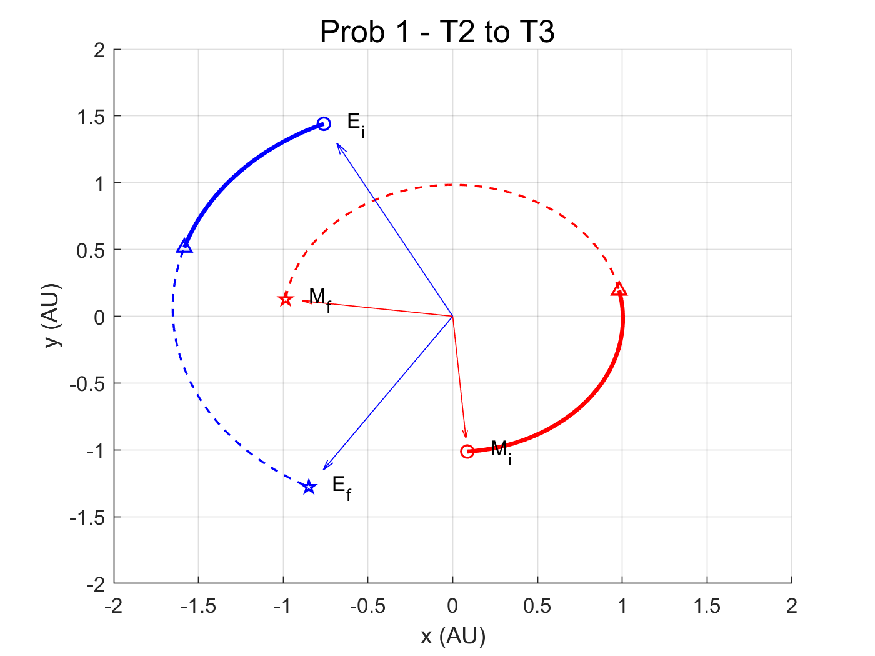
\includegraphics[width=0.7\textwidth]{Prob 1 - T2 to T3.pdf}
    \caption{Mars to Earth 60 degrees inbound transfer}
\end{figure}


% \newpage 
% ================================================================ % 
\section*{Problem 2}

\subsection*{A}
In the previous section, the 

% ------------------------- % 
\subsection*{B}


% ------------------------- % 
\subsection*{C}


\newpage
% ================================================================ % 
\section*{Appendix} 

\subsection*{MATLAB code} 

\begin{lstlisting}

    
	
\end{lstlisting}





% ================================================================ % 

% \bibliography{sample}

\end{document}
